
\documentclass[11pt,a4paper]{article}
\usepackage{ucs}
\usepackage[utf8x]{inputenc}
\usepackage[T1]{fontenc}
\usepackage{ngerman}
\usepackage{amsmath,amssymb,amstext}
\usepackage{tikz}
\title{Rechnerstrukturen Blatt 3}
\author{Sven Marquardt}
\date{\today}
\input{kvmacros}
\usetikzlibrary{automata}
\usetikzlibrary{positioning}
\usetikzlibrary{topaths}
\begin{document}
Aufgabe3.1\\
Die Schaltung soll einen Zähler darstellen, der in 3er Schritten vorwärts oder rückwärts zählt. Das Umstellen der Zählrichtung erfolgt durch den Schalter $x_0$.\\
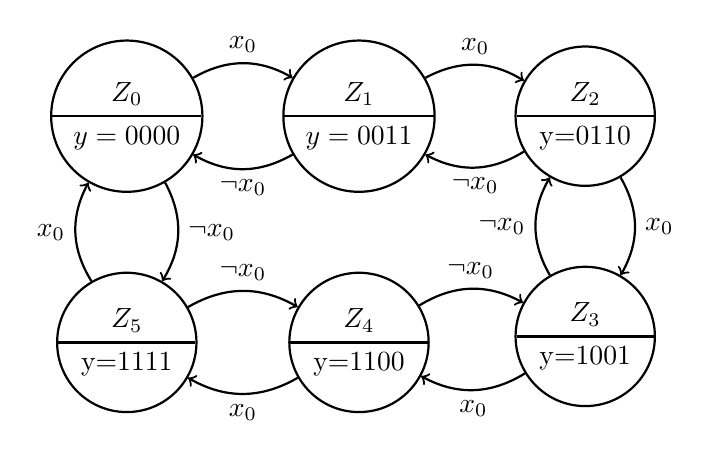
\begin{tikzpicture}[auto,thick]
	\node[state with output] (Z0) {$Z_0$ \nodepart {lower} $y=0000$};
	\node[state with output, right=of Z0] (Z1) {$Z_1$ \nodepart {lower} $y=0011$};
	\node[state with output, right=of Z1] (Z2) {$Z_2$ \nodepart {lower} y=0110};
	\node[state with output, below=of Z2] (Z3) {$Z_3$ \nodepart {lower} y=1001};
	\node[state with output, below=of Z1] (Z4) {$Z_4$ \nodepart {lower} y=1100};
	\node[state with output, below=of Z0] (Z5) {$Z_5$ \nodepart {lower} y=1111};
	\path[->] (Z0)	edge [bend left]		node	{$x_0$}(Z1)
			  		edge [bend left]		node[right]	{$\neg x_0$}(Z5)
			  (Z1)	edge [bend left]		node	{$\neg x_0$}(Z0)
			  		edge [bend left]		node	{$x_0$}(Z2)
			  (Z2)	edge [bend left]		node	{$\neg x_0$}(Z1)
			  		edge [bend left]		node	{$x_0$}(Z3)
			  (Z3)	edge [bend left]		node	{$\neg x_0$}(Z2)
			  		edge [bend left]		node	{$x_0$}(Z4)
			  (Z4)	edge [bend left]		node	{$\neg x_0$}(Z3)
			  		edge [bend left]		node	{$x_0$}(Z5)
			  (Z5)	edge [bend left]		node[left]	{$x_0$}(Z0)			  		
			  		edge [bend left]		node	{$\neg x_0$}(Z4);
\end{tikzpicture}
\\
A=$ ( X,Y,Z, \delta, \mu ) $ ,mit\\
$X= \lbrace 0,1 \rbrace$\\
$Y= \lbrace 0000,0011,0110,1001,1100,1111 \rbrace$\\
$Z= \lbrace 000,001,010,011,100,101 \rbrace$\\
$\delta : Z \times X \rightarrow Z$\\
$\mu : Z \rightarrow Y$\\ \\
Dazu die Wertetabelle \\ \\
\begin{tabular}{c | c | c | c | c | | c | c | c | c | | c | c | c | c}
$x_0$&Z&$z_2$&$z_1$&$z_0$&$y_3$&$y_2$&$y_1$&$y_0$&$Z^+$&$z^+_2$&$z^+_1$&$z^+_0$ \\ \hline
0&$Z_0$&0&0&0&0&0&0&0&$Z_1$&0&0&1\\
0&$Z_1$&0&0&1&0&0&1&1&$Z_2$&0&1&0\\
0&$Z_2$&0&1&0&0&1&1&0&$Z_3$&0&1&1\\
0&$Z_3$&0&1&1&1&0&0&1&$Z_4$&1&0&0\\
0&$Z_4$&1&0&0&1&1&0&0&$Z_5$&1&0&1\\
0&$Z_5$&1&0&1&1&1&1&1&$Z_0$&0&0&0\\
0&--&1&1&0&*&*&*&*&--&*&*&*\\
0&--&1&1&1&*&*&*&*&--&*&*&*\\ \hline
1&$Z_0$&0&0&0&0&0&0&0&$Z_5$&1&0&1\\
1&$Z_1$&0&0&1&0&0&1&1&$Z_0$&0&0&0\\
1&$Z_2$&0&1&0&0&1&1&0&$Z_1$&0&0&1\\
1&$Z_3$&0&1&1&1&0&0&1&$Z_2$&0&1&0\\
1&$Z_4$&1&0&0&1&1&0&0&$Z_3$&0&1&1\\
1&$Z_5$&1&0&1&1&1&1&1&$Z_4$&1&0&0\\
1&--&1&1&0&*&*&*&*&--&*&*&*\\
1&--&1&1&1&*&*&*&*&--&*&*&*\\
\end{tabular}\\
\\ \\  \\
Daraus ergeben sich folgende KV-Diagramme für $z^+_2,z^+_1$ und $z^+_0$.\\
\karnaughmap{4}{$z^+_2$}{{$x_0$}{$z_2$}{$z_1$}{$z_0$}}{000110**100001**}{
\textcolor{blue}{
\put(3.5,3){\oval(1.0,1.9)[]}}
\textcolor{red}{
\put(1.85,2.5){\oval(1.9,1.0)[]}}
\textcolor{black}{
\put(0.2,0.5){\oval(1.0,1.0)[]}}
\textcolor{green}{
\put(2,1){\oval(1.0,1.9)[]}}
}\\
$z^+_2=\textcolor{blue}{ (\neg z_0 \wedge z_2 \wedge \neg x_0 ) } \vee \textcolor{red}{(z_0 \wedge z_1 \wedge \neg x_0)} \vee \textcolor{green}{(z_0 \wedge z_2 \wedge x_0)} \vee \textcolor{black}{ ( \neg z_0 \wedge \neg z_1 \wedge \neg z_2 \wedge x_0)}$\\
\karnaughmap{4}{$z^+_1$}{{$x_0$}{$z_2$}{$z_1$}{$z_0$}}{011000**000101**}{
\textcolor{red}{
\put(1.5,3.5){\oval(1.0,1.0)[]}
}
\textcolor{blue}{
\put(-0.15,2.5){\oval(1.8,0.9)[r]}
\put(3.85,2.5){\oval(1.8,0.9)[l]}
}
\textcolor{green}{
\put(1.7,1.5){\oval(1.9,0.9)[]}}
\textcolor{black}{
\put(2,1){\oval(0.9,1.9)[]}}
}\\
$z^+_1= \textcolor{red}{(z_0 \wedge \neg z_1 \wedge \neg z_2 \wedge \neg x_0)} \vee \textcolor{blue}{(\neg z_0 \wedge z_1 \wedge \neg x_0)} \vee \textcolor{green}{(z_0 \wedge z_1 \wedge x_0)} \vee (z_0 \wedge z_2 \wedge x_0)$\\
\karnaughmap{4}{$z^+_0$}{{$x_0$}{$z_2$}{$z_1$}{$z_0$}}{101010**101010**}{
\textcolor{red}{
\put(-0.04,1.95){\oval(2,3.9)[r]}
\put(4.04,1.95){\oval(2.01,3.9)[l]}
}
}
$z^+_0=\textcolor{red}{\neg z_0}$\\ 
Folglich bilden folgende KV-Diagramme die Minimierung der Ausgangsfunktion.\\
\kvunitlength=5mm
\karnaughmap{3}{$y_3$}{{$z_2$}{$z_1$}{$z_0$}}{000111**}{
\textcolor{red}{
\put(3,1){\oval(2,2)}}
\textcolor{blue}{
\put(1.85,0.5){\oval(2,1)}}
}
$y_3= \textcolor{red}{z_2} \vee \textcolor{blue}{(z_0 \wedge z_1)}$
\karnaughmap{3}{$y_2$}{{$z_2$}{$z_1$}{$z_0$}}{001011**}{
\textcolor{red}{
\put(3,1){\oval(2,2)}}
\textcolor{blue}{
\put(-0.15,0.5){\oval(2,0.9)[r]}
\put(3.85,0.5){\oval(2,0.9)[l]}}
}
$y_2= \textcolor{red}{z_2} \vee \textcolor{blue}{ ( \neg z_0 \wedge z_1)}$\\
\karnaughmap{3}{$y_1$}{{$z_2$}{$z_1$}{$z_0$}}{011001**}{
\textcolor{red}{
\put(2,1.5){\oval(2,1)}}
\textcolor{blue}{
\put(-0.15,0.5){\oval(2,0.9)[r]}
\put(3.85,0.5){\oval(2,0.9)[l]}}}
$y_1=\textcolor{red}{(z_0 \wedge \neg z_1)} \vee \textcolor{blue}{(\neg z_0 \wedge z_1)}$
\karnaughmap{3}{$y_0$}{{$z_2$}{$z_1$}{$z_0$}}{010101**}{
\textcolor{red}{
\put(2,1){\oval(2,2)}}}
$y_0=\textcolor{red}{z_0}$\\ \\ \\

Aufgabe 3.2\\
In dieser Aufgabe soll eine Ampel implementiert werden, die automatisch läuft. Heißt, nach einer gewissen Zeit gibt es automatisch Grün für die Fußgänger, ohne dass ein Knopf gedrückt werden muss. Es ist also ein autonomer Automat. Folglich beschreibt folgender Automat die Funktion der Ampel. \\
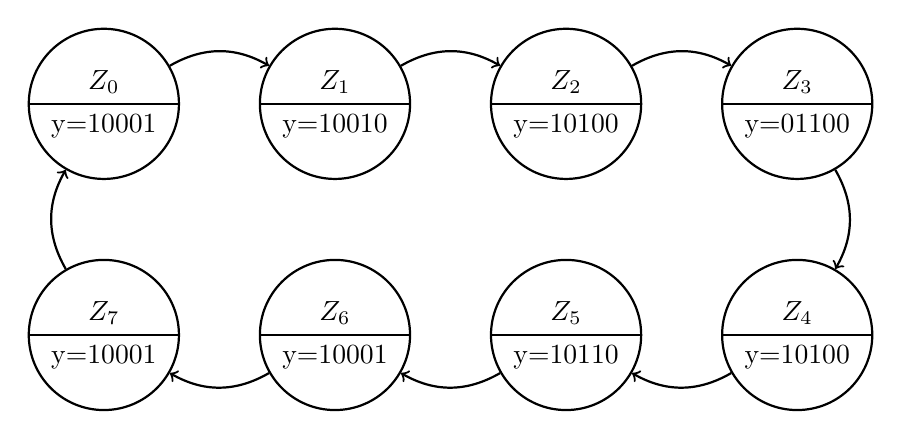
\begin{tikzpicture}[auto,thick]
	\node[state with output] (Z0) {$Z_0$ \nodepart {lower} y=10001};
	\node[state with output, right=of Z0] (Z1) {$Z_1$ \nodepart {lower} y=10010};
	\node[state with output, right=of Z1] (Z2) {$Z_2$ \nodepart {lower} y=10100};
	\node[state with output, right=of Z2] (Z3) {$Z_3$ \nodepart {lower} y=01100};
	\node[state with output, below=of Z3] (Z4) {$Z_4$ \nodepart {lower} y=10100};
	\node[state with output, below=of Z2] (Z5) {$Z_5$ \nodepart {lower} y=10110};
	\node[state with output, below=of Z1] (Z6) {$Z_6$ \nodepart {lower} y=10001};
	\node[state with output, below=of Z0] (Z7) {$Z_7$ \nodepart {lower} y=10001};
	\path[->]
	(Z0)	edge [bend left]	node{}	(Z1)
	(Z1)	edge [bend left]	node{}	(Z2)
	(Z2)	edge [bend left]	node{}	(Z3)
	(Z3)	edge [bend left]	node{}	(Z4)
	(Z4)	edge [bend left]	node{}	(Z5)
	(Z5)	edge [bend left]	node{}	(Z6)
	(Z6)	edge [bend left]	node{}	(Z7)
	(Z7)	edge [bend left]	node{}	(Z0);
\end{tikzpicture}\\ \\
$A= (Y,Z,\delta,\mu)$ , mit\\
$Y= \lbrace 10001,10010,10100,01100,10110 \rbrace$ \\
$Z=\lbrace 000,001,010,011,100,101,110,111 \rbrace$ \\
$\delta : Z \rightarrow Z$\\
$\mu : Z \rightarrow Y$\\
\begin{tabular}{ c | c | c | c | | c | c | c | | c | c | c | c | c | c | | c | c | c | c | c}
Z&$z_2$&$z_1$&$z_0$&$z^+_2$&$z^+_1$&$z^+_0$&$J_2$&$K_2$&$J_1$&$K_1$&$J_0$&$K_0$&$y_4$&$y_3$&$y_2$&$y_1$&$y_0$ \\ \hline
$Z_0$&0&0&0&0&0&1&0&*&0&*&1&*&1&0&0&0&1\\
$Z_1$&0&0&1&0&1&0&0&*&1&*&*&1&1&0&0&1&0\\
$Z_2$&0&1&0&0&1&1&0&*&*&0&1&*&1&0&1&0&0\\
$Z_3$&0&1&1&1&0&0&1&*&*&1&*&1&0&1&1&0&0\\
$Z_4$&1&0&0&1&0&1&*&0&0&*&1&*&1&0&1&0&0\\
$Z_5$&1&0&1&1&1&0&*&0&1&*&*&1&1&0&1&1&0\\
$Z_6$&1&1&0&1&1&1&*&0&*&0&1&*&1&0&0&0&1\\
$Z_7$&1&1&1&0&0&0&*&1&*&1&*&1&1&0&0&0&1\\ \hline
\end{tabular}\\ \\ \\ \\ \\ \\ \\
Die Minimierung der Zustandsübergangsfunktion \\
\karnaughmap{3}{$J_2$}{{$z_2$}{$z_1$}{$z_0$}}{0001****}{
\textcolor{red}{
\put(2,0.5){\oval(1.9,0.9)}}}
$J_2= \textcolor{red}{z_0 \wedge z_1}$
\karnaughmap{3}{$K_3$}{{$z_2$}{$z_1$}{$z_0$}}{****0001}{
\textcolor{red}{
\put(2,0.5){\oval(1.9,0.9)}}}$K_2= \textcolor{red}{z_0 \wedge z_1}$\\
\karnaughmap{3}{$J_1$}{{$z_2$}{$z_1$}{$z_0$}}{01**01**}{
\textcolor{red}{
\put(2,1){\oval(2,2)}}}
$J_1= \textcolor{red}{z_0}$
\karnaughmap{3}{$K_1$}{{$z_2$}{$z_1$}{$z_0$}}{**01**01}{
\textcolor{red}{
\put(2,1){\oval(2,2)}}}
$K_1= \textcolor{red}{z_0}$\\
\karnaughmap{3}{$J_0$}{{$z_2$}{$z_1$}{$z_0$}}{1*1*1*1*}{
\textcolor{red}{
\put(2,1){\oval(4,2)}}} $J_0= \textcolor{red}{1}$
\karnaughmap{3}{$K_0$}{{$z_2$}{$z_1$}{$z_0$}}{*1*1*1*1}{\textcolor{red}{
\put(2,1){\oval(4,2)}}} $K_0= \textcolor{red}{1}$\\ \\
\karnaughmap{3}{$y_4$}{{$z_2$}{$z_1$}{$z_0$}}{11110111}{
\textcolor{red}{
\put(1,1){\oval(2,2)}}
\textcolor{blue}{
\put(1.8,1){\oval(2,2)}}
\textcolor{green}{
\put(2.5,0.5){\oval(1.9,1)}}}$y_4= \textcolor{red}{ \neg z_2} \vee \textcolor{blue}{z_0} \vee \textcolor{green}{(z_1 \wedge z_2)}$\\
\karnaughmap{3}{$y_3$}{{$z_2$}{$z_1$}{$z_0$}}{00001000}{
\textcolor{red}{
\put(3.5,1.5){\oval(1,1)}}}$y_3= \textcolor{red}{ \neg z_0 \wedge \neg z_1 \wedge z_2}$\\
\karnaughmap{3}{$y_2$}{{$z_2$}{$z_1$}{$z_0$}}{00011110}{
\textcolor{red}{
\put(3,1.5){\oval(1.9,1)}}
\textcolor{blue}{
\put(3.25,1){\oval(1,2)}}
\textcolor{green}{
\put(1,0.5){\oval(1,1)}}} $y_2= \textcolor{red}{( \neg z_1 \wedge z_2)} \vee \textcolor{blue}{( \neg z_0 \wedge z_2)} \vee \textcolor{green}{(z_0 \wedge z_1 \wedge \neg z_2)}$\\
\karnaughmap{3}{$y_1$}{{$z_2$}{$z_1$}{$z_0$}}{00100010}{
\textcolor{red}{
\put(0,0.5){\oval(1.9,1)[r]}
\put(4,0.5){\oval(1.9,1)[l]}
}}
$y_1= \textcolor{red}{ \neg z_0 \wedge z_1 }$\\
\karnaughmap{3}{$y_0$}{{$z_2$}{$z_1$}{$z_0$}}{11000001}{
\textcolor{red}{
\put(1,1.5){\oval(2,1)}
}
\textcolor{blue}{
\put(2.3,0.5){\oval(1,0.9)}
}}$y_0= \textcolor{red}{( \neg z_1 \wedge \neg z_2)} \vee \textcolor{blue}{(z_0 \wedge z_1 \wedge z_2)}$

Aufgabe 3.3\\
In dieser Aufgabe soll die Ampelschaltung von 3.2 um einen Bedarfsknopf erweitert werden. Die Ampel der Fußgänger soll nun nur Grün zeigen, wenn zuvor ein Schalter betätigt wurde. Ohne Betätigen des Schalters bleibt der Zustand der Ampel für die Fußgänger auf Rot und für die Autofahrer auf Grün. Folgender Automat beschreibt die Ampel.\\ 
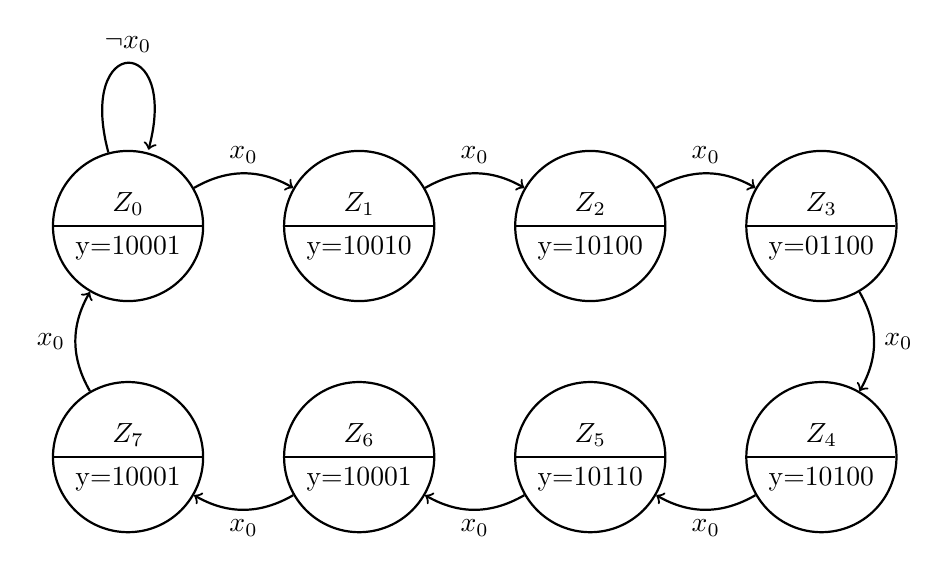
\begin{tikzpicture}[auto,thick]
	\node[state with output] (Z0) {$Z_0$ \nodepart {lower} y=10001};
	\node[state with output, right=of Z0] (Z1) {$Z_1$ \nodepart {lower} y=10010};
	\node[state with output, right=of Z1] (Z2) {$Z_2$ \nodepart {lower} y=10100};
	\node[state with output, right=of Z2] (Z3) {$Z_3$ \nodepart {lower} y=01100};
	\node[state with output, below=of Z3] (Z4) {$Z_4$ \nodepart {lower} y=10100};
	\node[state with output, below=of Z2] (Z5) {$Z_5$ \nodepart {lower} y=10110};
	\node[state with output, below=of Z1] (Z6) {$Z_6$ \nodepart {lower} y=10001};
	\node[state with output, below=of Z0] (Z7) {$Z_7$ \nodepart {lower} y=10001};
	\path[->]
	(Z0)	edge [bend left]	node{$x_0$}	(Z1)
	(Z0)	edge [loop above]			node[swap]{$\neg x_0$}	()
	(Z1)	edge [bend left]	node{$x_0$}	(Z2)
	(Z2)	edge [bend left]	node{$x_0$}	(Z3)
	(Z3)	edge [bend left]	node{$x_0$}	(Z4)
	(Z4)	edge [bend left]	node{$x_0$}	(Z5)
	(Z5)	edge [bend left]	node{$x_0$}	(Z6)
	(Z6)	edge [bend left]	node{$x_0$}	(Z7)
	(Z7)	edge [bend left]	node{$x_0$}	(Z0);
\end{tikzpicture}\\ \\ 
$A=(X,Y,Z, \delta, \mu )$, mit\\
$X=\lbrace 0,1 \rbrace$\\
$Y= \lbrace 10001,10010,10110,01100,10100 \rbrace$\\
$Z=\lbrace 000,001,010,011,100,101,110,111 \rbrace$ \\
$\delta : Z \times X \rightarrow Z$\\
$\mu : Z \rightarrow Y$\\ \\
Die Wertetabelle dazu\\
\begin{tabular}{c | c | c | c | c | | c | c | c | | c | c | c | c | c | c | | c | c | c | c | c}
$x_0$&Z&$z_2$&$z_1$&$z_0$&$z^+_2$&$z^+_1$&$z^+_0$&$J_2$&$K_2$&$J_1$&$K_1$&$J_0$&$K_0$&$y_4$&$y_3$&$y_2$&$y_1$&$y_0$ \\ \hline
0&$Z_0$&0&0&0&0&0&0&0&*&0&*&0&*&1&0&0&0&1\\
0&$Z_1$&0&0&1&0&1&0&0&*&1&*&*&1&1&0&0&0&1\\
0&$Z_2$&0&1&0&0&1&1&0&*&*&0&1&*&1&0&0&0&1\\
0&$Z_3$&0&1&1&1&0&0&1&*&*&1&*&1&1&0&0&0&1\\
0&$Z_4$&1&0&0&1&0&1&*&0&0&*&1&*&1&0&0&0&1\\
0&$Z_5$&1&0&1&1&1&0&*&0&1&*&*&1&1&0&0&1&1\\
0&$Z_6$&1&1&0&1&1&1&*&0&*&0&1&*&1&0&0&0&1\\
0&$Z_7$&1&1&1&0&0&0&*&1&*&1&*&1&1&0&0&0&1\\ \hline
1&$Z_0$&0&0&0&0&0&1&0&*&0&*&1&*&1&0&0&0&1\\
1&$Z_1$&0&0&1&0&1&0&0&*&1&*&*&1&1&0&0&1&0\\
1&$Z_2$&0&1&0&0&1&1&0&*&*&0&1&*&1&0&1&0&0\\
1&$Z_3$&0&1&1&1&0&0&1&*&*&1&*&1&0&1&1&0&0\\
1&$Z_4$&1&0&0&1&0&1&*&0&0&*&1&*&1&0&1&0&0\\
1&$Z_5$&1&0&1&1&1&0&*&0&1&*&*&1&1&0&1&1&0\\
1&$Z_6$&1&1&0&1&1&1&*&0&*&0&1&*&1&0&0&0&1\\
1&$Z_7$&1&1&1&0&0&0&*&1&*&1&*&1&1&0&0&0&1\\
\end{tabular}\\ \\
\karnaughmap{4}{$J_2$}{{$x_0$}{$z_2$}{$z_1$}{$z_0$}}{0001****0001****}{\textcolor{red}{
\put(2,2){\oval(2,2)}}}
$J_2= \textcolor{red}{z_0 \wedge z_1}$
\karnaughmap{4}{$K_2$}{{$x_0$}{$z_2$}{$z_1$}{$z_0$}}{****0001****0001}{\textcolor{red}{
\put(2,2){\oval(2,2)}}}$K_2= \textcolor{red}{z_0 \wedge z_1}$\\\\
\karnaughmap{4}{$J_1$}{{$x_0$}{$z_2$}{$z_1$}{$z_0$}}{01**01**01**01**}{\textcolor{red}{
\put(2,2){\oval(1.9,4)}}}
$J_1= \textcolor{red}{z_0}$
\karnaughmap{4}{$K_1$}{{$z_2$}{$z_1$}{$z_0$}}{**01**01**01**01}{\textcolor{red}{
\put(2,2){\oval(1.9,4)}}}
$K_1= \textcolor{red}{z_0}$\\
\karnaughmap{4}{$J_0$}{{$x_0$}{$z_2$}{$z_1$}{$z_0$}}{0*1*1*1*1*1*1*1*}{
\textcolor{red}{
\put(3,2){\oval(1.9,4)}
}
\textcolor{blue}{
\put(1.75,2){\oval(4,1.9)}
}\textcolor{green}{
\put(1.75,1){\oval(4,1.9)}
}}
$J_0= \textcolor{red}{z_2} \vee \textcolor{blue}{z_1} \vee \textcolor{green}{x_0}$
\karnaughmap{4}{$K_0$}{{$x_0$}{$z_2$}{$z_1$}{$z_0$}}{*1*1*1*1*1*1*1*1}{
\textcolor{red}{
\put(2,2){\oval(4,4)}
}} $K_0= \textcolor{red}{1}$ \\ 
\karnaughmap{3}{$y_4$}{{$z_2$}{$z_1$}{$z_0$}}{11110111}{
\textcolor{red}{
\put(1,1){\oval(2,2)}}
\textcolor{blue}{
\put(1.8,1){\oval(2,2)}}
\textcolor{green}{
\put(2.5,0.5){\oval(1.9,1)}}}$y_4= \textcolor{red}{ \neg z_2} \vee \textcolor{blue}{z_0} \vee \textcolor{green}{(z_1 \wedge z_2)}$\\
\karnaughmap{3}{$y_3$}{{$z_2$}{$z_1$}{$z_0$}}{00001000}{
\textcolor{red}{
\put(3.5,1.5){\oval(1,1)}}}$y_3= \textcolor{red}{ \neg z_0 \wedge \neg z_1 \wedge z_2}$\\
\karnaughmap{3}{$y_2$}{{$z_2$}{$z_1$}{$z_0$}}{00011110}{
\textcolor{red}{
\put(3,1.5){\oval(1.9,1)}}
\textcolor{blue}{
\put(3.25,1){\oval(1,2)}}
\textcolor{green}{
\put(1,0.5){\oval(1,1)}}} $y_2= \textcolor{red}{( \neg z_1 \wedge z_2)} \vee \textcolor{blue}{( \neg z_0 \wedge z_2)} \vee \textcolor{green}{(z_0 \wedge z_1 \wedge \neg z_2)}$\\
\karnaughmap{3}{$y_1$}{{$z_2$}{$z_1$}{$z_0$}}{00100010}{
\textcolor{red}{
\put(0,0.5){\oval(1.9,1)[r]}
\put(4,0.5){\oval(1.9,1)[l]}
}}
$y_1= \textcolor{red}{ \neg z_0 \wedge z_1 }$\\
\karnaughmap{3}{$y_0$}{{$z_2$}{$z_1$}{$z_0$}}{11000001}{
\textcolor{red}{
\put(1,1.5){\oval(2,1)}
}
\textcolor{blue}{
\put(2.3,0.5){\oval(1,0.9)}
}}$y_0= \textcolor{red}{( \neg z_1 \wedge \neg z_2)} \vee \textcolor{blue}{(z_0 \wedge z_1 \wedge z_2)}$

\end{document}
